%
% $Id: main.tex 14 2014-02-04 22:36:30Z nicb $
%
\newcommand{\topic}{Campionamento, Sintesi ed Elaborazione dei Segnali Musicali\xspace}
\newcommand{\topicacro}{CSEDSM\xspace}
\newcommand{\level}{II\xspace}
\documentclass{scrbook}
\usepackage[italian]{babel}
\usepackage{svninfo}
\usepackage{fancyvrb}
\usepackage{paralist}
\usepackage[italian]{varioref}
\usepackage{nesse}
\usepackage{xspace}
\usepackage{nicefrac}

\newcommand{\rootdir}{..}
\newcommand{\imagedir}{\rootdir/images}
\newcommand{\plotdir}{\rootdir/plots}
\newcommand{\rcstag}{ver.\svnInfoRevision\ \svnInfoDate\xspace}
\title{\topic (\topicacro) \level\\dispense\\{\tiny (\rcstag)}}
\author{Nicola Bernardini}
\date{~}

\setlength{\parsep}{2\baselineskip}
\setlength{\parindent}{0pt}

\begin{document}
\svnInfo $Id: main.tex 14 2014-02-04 22:36:30Z nicb $

\maketitle

\tableofcontents

%
% $Id: introduction.tex 14 2014-02-04 22:36:30Z nicb $
%

\chapter{Introduzione}

Queste sono le dispense della seconda annualit\`a dell'insegnamento di \emph{topic}
(aka \emph{\topicacro}) tenuto da Nicola Bernardini nell'A.A 2012-2013 al
Conservatorio ``C.Pollini'' di Padova.

Queste dispense sono tratte in larga parte da alcuni capitoli di \emph{A Digital Signal Processing Primer}
di Ken Steiglitz \cite{steiglitz:adspp} - integrati
con spiegazioni supplementari laddove l'aspetto matematico \`e un po' pi\`u
difficile,
e con materiali elaborati in
classe dagli studenti
nonch\'e tratti da altri testi
(cf. \cite{steiglitz1974, t1987digital, park2010, shenoi2005}).

\chapter{Un ripasso dei filtri FIR\label{chap:fir}}
%
% $Id: ripasso_FIR.tex 14 2014-02-04 22:36:30Z nicb $
%
\svnInfo $Id: ripasso_FIR.tex 14 2014-02-04 22:36:30Z nicb $

\section{Trasformata zeta applicata ai filtri FIR\label{sec:zeta fir}}

\subsection{Ritardo e linearit\`a\label{sec:ritardo e linearita}}

Recuperiamo le propriet\`a della trasformata Z e applichiamole ai filtri FIR.

\begin{itemize}

\item filtro FIR:
				
		\begin{equation}
			X(k)\,\raiseto{H}\,Y(k)
		\end{equation}

		La forma generalizzata di un filtro FIR \`e:
  
		\begin{equation}
    	Y(k) = C(1)X(k) + C(2)X(k-1) + ... + C(M)X(k-M+1)
		\end{equation}

\item per via della propriet\`a 2 della trasformata Z (linearit\`a) la trasformata Z di questa somma
     \`e uguale alla somma delle trasformata Z di ogni termine. Per via della propriet\`a
     1, ciascun termine pu\`o essere letto come multiplo della trasformata Z di $X(k)$,
     perch\'e:
 
		 \begin{equation}
			 \begin{array}{r c l}
						 C(1)X(k) & \raiseto{Z} & C(1)X^{*}(z)\\
						 C(2)X(k-1) & \raiseto{Z} & C(2)z^{-1}X^{*}(z)\\
						 C(3)X(k-2) & \raiseto{Z} & C(3)z^{-2}X^{*}(z)\\
						            & \vdots & \\
						 C(M)X(k-M+1) & \raiseto{Z} & C(M)z^{(-M+1)}X^{*}(z)\\
		    \end{array}
		 \end{equation}
 
     quindi:

		 \begin{equation}
						 Y(k)\,\raiseto{Z}\,Y^{*}(z) = [ C(1)+C(2)z^{-1}+C(2)z^{-2}+ \ldots +C(M)z^{-(M+1)} ] X^{*}(z)
		 \end{equation}
 
		 ponendo
 
		 \begin{equation}
			 H(z) = [ C(1)+C(2)z^{-1}+C(2)z^{-2}+ \ldots +C(M)z^{-(M+1)} ]
		 \end{equation}
 
     ossia
 
		 \begin{equation}
						 H(z) = \frac{Y^{*}(z)}{X^{*}(z)}
		 \end{equation}
 
\item quindi: quando $X$ \`e un fasore, anche $Y$ \`e un fasore e il rapporto tra $X$ e
			$Y$ \`e proprio $H(z)$ (quando $z = e^{i\omega}$): quando io metto dentro al filtro un
      segnale sinusoidale ottengo un segnale sinusoidale riscalato

\item ma la faccenda \`e molto pi\`u generale: quando X  \`e  un  qualsiasi
      segnale causale (one-sided), l'uscita di un black box pu\`o  essere
      ottenuta semplicemente moltiplicando la sua trasformata $Z$  per  la
      funzione di trasferimento $H(z)$
 
			\begin{itemize}

			\item facciamo un esempio semplice:
 
				\begin{equation}
	 			\begin{array}{c c c l}
	  			X(k) & = & 0  & \quad per~k~<~0\\
         X(0) & = & 1  &          \\
         X(1) & = & 1  &          \\
				 X(k) & = & 0  & \quad per~k~>~1\\
					\end{array}
			 \end{equation}
 
 \item dalla definizione di trasformata Z ($X^{*}(z) = \sum_0^{N}{X(n)z^{-n}}$), la trasformata di questo segnale \`e:

				 \begin{equation}
								 X^{*}(z) = 1 + z^{-1}
				 \end{equation}
 
 \item ora filtriamolo col solito filtro di media semplicissimo:
 
		 		\begin{equation}
        	 Y(k) = X(k) + X(k-1)
		    \end{equation}
 
 \item la funzione di trasferimento \`e:
 
		 \begin{equation}
						 H(z) = 1 + z^{-1}
		 \end{equation}
 
 \item quindi:
 
		 \begin{equation}
						 Y^{*}(z) = H(z)X^{*}(z) = (1+z^{-1})(1+z^{-1}) = 1 + 2 z^{-1} + z^{-2}
		 \end{equation}

 \item \`e facile fare la trasformata inversa perch\'e ci sono tutte potenze decrescenti
       di zeta, quindi:
 
			 	\begin{equation}
								\begin{array}{c c c l}
           Y(k) & = & 0 & per\,k\,<\,0 \\
           Y(0) & = & 1 & \\
           Y(1) & = & 2 & \\
           Y(2) & = & 1 & \\
           Y(k) & = & 0 & per\,k\,>\,2\\
								\end{array}
		 \end{equation}
 
       si pu\`o verificare la correttezza facendo girare ``a mano'' il filtro

			\end{itemize}
%
%    - dimostrare che la trasformata Z \`e unica per ogni segnale, cio\`e che se due
%      segnali hanno la stessa trasformata Z, allora sono identici
%

\end{itemize}

\paragraph{Esercizi}

\begin{itemize}
 
 \item rifare il filtraggio sopra esposto con il seguente segnale:

				 \begin{equation}
						X(x) = \left\{
						   \begin{array}{c l}
									1 & 0 <= k <= 10 (o\,\,anche\,<=\,5)\\
									0 & altrimenti\\
							 \end{array} \right.
		     \end{equation}
 
       e con le seguenti funzioni di trasferimento:
 
			 	\begin{equation}
					\begin{array}{c c c c c}
	  				H(z) & = & 1 & - & z^{-1}\\
						 H(z) & = & 1 & + & z^{-1}\\
             H(z) & = & ( 1 & - & z^{-1} )^2\\
	      	 \end{array}
	       \end{equation}

\end{itemize}

\section{Una collezione di trasformate zeta notevoli\label{sec:zeta notevoli}}

\subsection{La trasformata zeta pi\`u semplice}

		La trasformata pi\`u semplice \`e quella che prevede campioni  non  zero  per  un
     numero finito di campioni. Per come abbiamo visto l'altra volta, la
     trasformata  $Z$  di  un  segnale  del  genere  \`e  semplicemente  un
     polinomio in $z^{-1}$. P.es.:

		 \begin{equation}
				X(k) = \left\{
					\begin{array}{c c c c}
						0 & k & <= & 0\\
						.5 & k & = & 1\\
						1 & k & = & 2\\
						.5 & k & = & 3\\
						0 & k & > & 3\\
		\end{array} \right.
		 \end{equation}

     Per la definizione di trasformata Z, la trasformata Z di questo segnale \`e

		 \begin{equation}
	   	 X^{*}(z) = .5z^{-1} + z^{-2} + .5z^{-3}
		 \end{equation}

     E la trasformata inversa \`e semplicemente la sequenza dei coefficienti del
     polinomio (== come se fossero ciascuno moltiplicato per 1)

\subsection{Un caso pi\`u interessante}

Un caso pi\`u interessante ha luogo quando il segnale \`e non  zero  per
    un infinito/indefinito numero  di  valori  di  k,  cio\`e  quando  il
    segnale va avanti per sempre. Questo a noi fa comodo per i segnali audio.
    Per noi p.es. sono molto importanti classi di segnali che sono
    esponenziali o sinusoidali di natura, e one-sided.

    Il segnale pi\`u semplice \`e la unit-step function in cui $X(k) = 1$ per $k >= 0$.
		La sua trasformata $z$ \`e:

		 \begin{equation}
						 X^{*}(z) = 1 + z^{-1} + z^{-2} + z^{-3} + \ldots
		 \end{equation}

    Questa \`e una serie geometrica ben conosciuta e sappiamo dall'algebra che
    la sua trasformata $z$ \`e quindi:

		 \begin{equation}
			 X^{*}(z) = \frac{1}{1-z^{-1}}
		 \end{equation}

   La serie geometrica funziona cos\`i: poniamo una serie

		 \begin{equation}
			a + ar + ar^{2} + ar^{3} + ... + ar^{n-1} = \sum_{k=0}^{n-1}{ar^{k}} =  \left\{ a\frac{1-r^{n}}{1 - r} \right\}
		 \end{equation}

   come ci si arriva? poniamo:

		 \begin{equation}
    s = a + ar + ar^{2} + \ldots + ar^{n-1}
		 \end{equation}

   allora 

		 \begin{equation}
    sr = ar + ar^{2} + ar^{3} + ... + ar^{n}
		 \end{equation}

   ma $s - sr = a - ar^{n}$, quindi $s(1 - r) = a(1 - r^{n})$, quindi

		 \begin{equation}
				s = a \frac{1 - r^{n}}{1 - r}
		 \end{equation}

   quando $n$ va all'infinito, \`e necessario che $r < 1$ per far convergere la somma. In questo caso

	 $\sum_{k=0}^{\inf}{ar^{k}}$ diventa $=\frac{a}{1 - r}$ e se $a = 1$, $= \frac{1}{1 - r}$

   quindi 

		 \begin{equation}
			  X^{*}(z) = \frac{1}{1-z^{-1}}
		 \end{equation}

   a patto che $|z^{-1}| < 1$ e dato che $|z^{-1}| = \frac{1}{|z|}$ questo equivale a dire che $|z| > 1$

   Se esaminiamo questo polinomio pi\`u da vicino, e moltiplichiamo num e den
   per $z$, questo diventa:

		 \begin{equation}
						 \frac{z}{z - 1}
		 \end{equation}

   e per $z = 1$, la trasformata zeta diventa infinita. Questo punto si chiama
	 un \emph{polo}. In questo caso quindi la trasformata $z$ ha uno zero per $z = 0$ e
	 un polo per $z = 1$. (un piano con uno zero al centro e un polo sul 1 reale -- cf.Fig.\vref{fig:poli e zeri}).
	 \begin{figure}[Hbtp]
			\begin{center}
				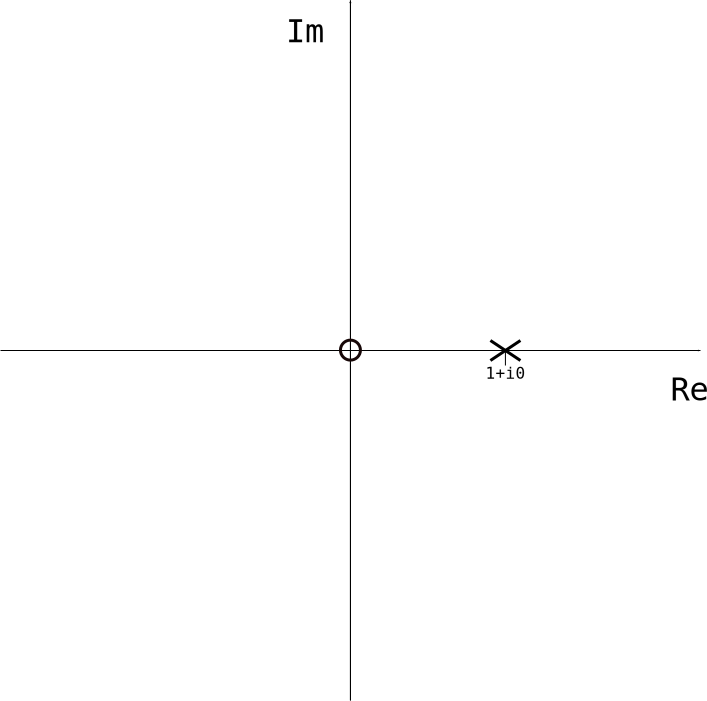
\includegraphics[width=0.35\textwidth]{\imagedir/piano_zeta_un_polo}
				\caption{Poli e zeri del filtro $X^{*}(z) = \frac{1}{1-z^{-1}}$\label{fig:poli e zeri}}
			\end{center}
	 \end{figure}
   Quindi a frequenza zero si sommano tutti gli uni e la somma infinita
   esplode. Possiamo trovare la magnitudine della trasformata $z$ sul cerchio
   unitario e questa si chiama ``contenuto frequenziale'' o \emph{risposta in
	 frequenza} del segnale. Ponendo $z = e^{-i\omega}$

		 \begin{equation}
				X^{*}(z) = \frac{1}{1 - e^{i\omega}}
		 \end{equation}

   la magnitudine (il modulo) \`e quindi:

		 \begin{equation}
				|X^{*}(z)| = \frac{1}{|1 - e^{i\omega}|}
		 \end{equation}


   e se moltiplico entrambi i membri del denominatore per $e^{-iw/2}$ ottengo

		 \begin{equation}
				 |X^{*}(z)| = \frac{1}{|e^{-i\omega/2} - e^{i\omega/2}|}
		 \end{equation}

   e quindi per via della formula di Eulero                 

	   \begin{equation}\label{eqn:infinitefir}
				 |X^{*}(z)| = \frac{1}{2 |sin {\omega/2}|}
		 \end{equation}
	\begin{figure}[htbp]	
		\begin{center}
			\includegraphics[width=0.4\textwidth]{\plotdir/infinitefir}
			\caption{Magnitudine dell'eq.\ref{eqn:infinitefir} con freq.  normalizzata}
		\end{center}
	\end{figure}


%
% $Id: IIR.tex 14 2014-02-04 22:36:30Z nicb $
%

\svnInfo $Id: IIR.tex 14 2014-02-04 22:36:30Z nicb $

\chapter{Filtri a feedback (IIR)\label{chap:iir}}

\section{Introduzione}

I filtri a feedback (IIR - per \emph{Infinite Impulse Response}) sono filtri nei quali vengono re-immessi in ingresso
versioni ritardate e riscalate dell'uscita.

Il filtro IIR pi\`u semplice \`e:

  \begin{equation}\label{eqn:filtro iir semplice}
		y_t = x_t + a_1 y_{t-1}
	\end{equation}

	In eq.\ref{eqn:filtro iir semplice} l'ultimo campione in uscita viene
	riscalato di un fattore $a_1$ e sommato di nuovo all'ingresso.

Potenzialmente la risposta di questo filtro a un impulso unitario \`e
infinita: p.es., introducendo un segnale consistente in un 1 al campione zero e zero
per tutti gli altri campioni all'interno di un filtro del genere con un
fattore $a_1 = 0.5$ otterremo in uscita:

  \begin{equation}
		y_t = 1, 0.5, 0.25, 0.125, 0.0625, \ldots
  \end{equation}

e cio\`e una risposta \emph{infinita}. Questo non pu\`o mai succedere con i
filtri FIR, la cui risposta \`e al massimo il numero dei campioni in ingresso
pi\`u il numero di campioni del filtro (i \emph{termini} meno uno.

L'altra differenza grossa con i filtri FIR \`e che gli IIR possono
letteralmente \emph{esplodere}. Per capire questo riprendiamo il filtro descritto in
\ref{eqn:filtro iir semplice} e poniamo il fattore $a_1 = 2$. L'uscita
numerica del
filtro sarà:

  \begin{equation}
		y_t = 1, 2, 4, 8, 16, \ldots
  \end{equation}

Essa diverger\`a all'infinito.

Per capire bene perch\'e, sostituiamo in eq.\ref{eqn:filtro iir semplice} a $y_t$ e $x_t$ (singoli campioni) i
vettori $Y$ e $X$ (che rappresentano ``interi segnali''):

  \begin{equation}\label{eqn:filtro iir segnali}
		Y = X + a_1 z^{-1} Y
	\end{equation}

	Se raggruppiamo i termini, l'eq.\ref{eqn:filtro iir segnali} diventa:

  \begin{equation}\label{eqn:filtro iir segnali raggruppata}
		X = Y - a_1 z^{-1} Y
	\end{equation}

Ma questa \`e l'equazione dei filtri FIR (feed--forward), solo che ingressi e
uscite sono scambiati. Sappiamo che la funzione di trasferimento del
corrispondente filtro FIR \`e:

	\begin{equation}
		1 - a_1 z^{-1}
	\end{equation}

e, dato che il caso del filtro IIR presenta l'equazione in forma invertita,
ossia:

	\begin{equation}
		X = H(z) Y
	\end{equation}

ovvero

	\begin{equation}
		Y = \frac{1}{H(z)} X
	\end{equation}

la funzione di trasferimento sar\`a quindi:

	\begin{equation}\label{eqn:iir tf}
		H(z) = \frac{1}{1 - a_1 z^{-1}}
	\end{equation}

La magnitudine della risposta in frequenza si otterr\`a come sempre
operando la sostituzione $z = e^{i\omega}$ e calcolando il modulo:

	\begin{equation}\label{eqn:iir tf 2}
		|H(z)| = \frac{1}{|1 - a_1 e^{-i\omega}|}
	\end{equation}

Quando $z = a_1$, $z^{-1} = \frac{1}{a_1}$, il denominatore
dell'eq.\ref{eqn:iir tf 2} diventa

	\begin{equation}\label{eqn:iir tf zero condition}
		1 - \frac{a_1}{a_1} = 1 - 1 = 0
	\end{equation}

e quindi in $a_1$ noi abbiamo un punto che diverge all'infinito. Quel punto si
chiama \emph{polo}.

Per calcolare bene la magnitudine della risposta sar\`a opportuno moltiplicare
numeratore e denominatore per $z$:

	\begin{equation}
		H(z) = \frac{1}{1 - a_1 z^{-1}} = \frac{z}{z - a_1}
	\end{equation}

Il modulo sar\`a

	\begin{equation}
		|H(z)| = \frac{|z|}{|z - a_1|}
	\end{equation}

	oss\`ia, sostituendo $z = e^{i\omega}$

	\begin{equation}\label{eqn:iir tf mag subst}
		|H(z)| = \frac{|e^{i\omega}|}{|e^{i\omega} - a_1|}
	\end{equation}

ma $|e^{i\omega}| = 1$ per qualsiasi $\omega$, quindi l'eq.\ref{eqn:iir tf mag subst}
diventa:

	\begin{equation}\label{eqn:iir tf mag subst no num}
		|H(z)| = \frac{1}{|e^{i\omega} - a_1|}
	\end{equation}

Scomponendo il denominatore in parte reale e parte immaginaria otteniamo

	\begin{equation}
		\begin{array}{l c l}
			Re_{den} & = & cos \omega - a_1\\
			Im_{den} & = & sin \omega\\
		\end{array}
	\end{equation}

e il modulo sar\`a quindi

	\begin{equation}
		|den| = \sqrt{( cos \omega - a_1 )^2 + ( sin \omega )^2}
	\end{equation}

ma

	\begin{equation}
		( cos \omega - a_1 )^2 = ( cos \omega - a_1 ) ( cos \omega - a_1 ) = cos^2 ( \omega ) - 2 a_1 cos ( \omega ) + a_1^2
	\end{equation}

e quindi

	\begin{equation}
		|den| = \sqrt{cos^2 ( \omega ) - 2 a_1 cos ( \omega ) + a_1^2 + sin^2 ( \omega )}
	\end{equation}

Ricordando che $cos^2 + sin^2 = 1$ per qualsiasi $\omega$, possiamo
semplificare:

	\begin{equation}
		|den| = \sqrt{1 - 2 a_1 cos ( \omega ) + a_1^2}
	\end{equation}

e l'eq.\ref{eqn:iir tf mag subst no num} diventa:

	\begin{equation}
		|H(z)| = \frac{1}{\sqrt{1 - 2 a_1 cos ( \omega ) + a_1^2}}
	\end{equation}

	\begin{figure}[htb]
		\begin{center}
			\includegraphics[width=0.6\textwidth]{\plotdir/iir3}
			\caption{Magnitudine (normalizzata a $0 dB$) del filtro IIR $\frac{1}{1 - a_1 z^{-1}}$\label{fig:simple IIR mag response}}
		\end{center}
	\end{figure}

	La figura \vref{fig:simple IIR mag response} illustra la magnitudine
	(normalizzata a $0 dB$) del nostro filtro con valori diversi di $a_1$.

\section{Risonanza e larghezza di banda\label{sec:resonance}}

\subsection{Risonanza e larghezza di banda di un filtro}
Dato che si tratta di una funzione continua, la larghezza di banda di un
  filtro \`e per definizione il punto in cui la potenza \`e dimezzata (cio\`e
	$1/\sqrt{2} = -3 dB$ -- cf.Fig.\vref{fig:bw})

	\begin{figure}[htb]
		\begin{center}
		  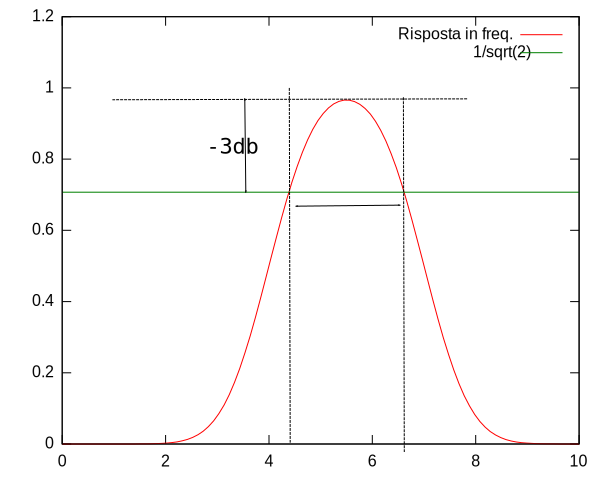
\includegraphics[width=0.6\textwidth]{\imagedir/bw}
		  \caption{Misurazione della larghezza di banda di un filtro\label{fig:bw}}
		\end{center}
	\end{figure}

	Quando un filtro ha un polo collocato da qualche parte sul piano $z$ questo
    polo avr\`a un modulo R e un angolo $\theta$.
  
	Consideriamo ora l'effetto di un polo sul cerchio unitario sull'asse reale:
    se $\theta$ \`e 0 avremo un filtro passa basso e l'algebra si semplifica. Se
    $\theta$ \`e non-zero l'effetto sar\`a uguale ruotato di un angolo
		$\theta$.
  
	Dato che per i fitri IIR a un polo la funzione di trasferimento \`e
  
		 \begin{equation}
				H(z) = \frac{1}{1 - a_1 z^{-1}}
		 \end{equation}

	l'inverso del quadrato della della risposta in magnitudine ad una frequenza
    $\psi (rad/campione)$ legata a questo polo sull'asse reale laddove $z = R$ \`e
  
		 \begin{equation}
				\frac{1}{|H(z)|^2} = |1 - a_1 z^{-1}|^2 = | z - a_1 |^2
		 \end{equation}
  
    ponendo $z = e^{i\theta}$ e $a_1 = R$
  
		 \begin{equation}
				\frac{1}{|H(z)|^2} =  |e^{i\theta} - R|^2
		 \end{equation}
  
    svolgendo il modulo
  
		 \begin{equation}
				\frac{1}{|H(z)|^2} =  1 - 2 R cos\,\theta + R^2
		 \end{equation}
  
	Nel centro della risonanza $\theta = 0$, $cos\,\theta = 1$ e l'equazione diventa:
  
		 \begin{equation}
				\frac{1}{|H(z)|^2} =  1 - 2 R cos\,\theta + R^2
		 \end{equation}

		 \begin{equation}
				\frac{1}{|H(z)|^2} =  1 - 2 R + R^2 = (1 - R)^2
		 \end{equation}

		cio\`e il quadrato della distanza tra
    la frequenza zero sul cerchio unitario $(z = 1)$ \`e il polo
  
  Per trovare i punti in cui la magnitudine \`e $1/\sqrt{2}$, guardiamo
    per quale $\theta$ la magnitudine \`e il doppio di questo, quindi:
  
		\begin{equation}\label{eqn:theta solution for bw}
    1 - 2 R cos \theta + R^2 = 2 (1 - R)^2 = 2 [ 1 - 2R + R^2 ]
		 \end{equation}
  
	Risolviamo quindi l'eq.\ref{eqn:theta solution for bw} per $\theta$:

	\begin{equation}
		- 2 R cos \theta = 2 - 4R + 2 R^2 - 1 - 2 R^2 = 1 - 4 R 
  \end{equation}

	ossia

	\begin{equation}
					cos \theta = -\frac{1}{2 R} + \frac{4 R}{2 R} = - \frac{1}{2R} + 2 R
  \end{equation}

	quindi

	\begin{equation}
		\theta = arccos \left ( 2 R  - \frac{1}{2 R} \right )
	\end{equation}

	%
	% VERIFICARE e inventare un PLOT che faccia vedere
	%
  
\section{Resons}
  
					I filtri a un polo hanno i poli e gli zeri che si dispongono
    soltanto a freq. zero o nyquist, a seconda del fatto che il polo sia pi\`u
    vicino a $z = +1$ o $z = -1$.
  
	Per avere filtri che risuonino ad una frequenza desiderata qualsiasi abbiamo
    (e per fare in modo che il filtro tiri fuori un segnale reale) ci vogliono
    almeno un paio di poli disposti in maniera complessa coniugata
  
		 \begin{equation}
						 H(z) = \frac{1}{(1 - Re^{i\theta} z^{-1})(1 - Re^{-i\theta} z^{-1})}
		 \end{equation}
  
    dove R \`e il modulo del polo e $\theta$ \`e l'angolo (frq) e $Re^{+/-\theta}$ sono le
    radici del denominatore (poli)
  
	Ora se eseguiamo la moltiplicazione del denominatore quello che otteniamo \`e:
  
		 \begin{equation}
			 \begin{array}{r c c c l c l}
     den & = & (1 & - & Re^{i\theta} z^{-1})(1 - Re^{-i\theta} z^{-1}) & &\\
         & = & 1 & - & Re^{-i\theta} z^{-1} - Re^{i\theta} z^{-1} & + & R^{2} z^{-2}\\
         & = & 1 & - & Rz^{-1} (e^{i\theta} + e^{-i\theta}) & + & R^{2} z^{-2}\\
         & = & 1 & - & Rz^{-1} 2 cos \theta & + & R^{2} z^{-2}\\
		 		\end{array}
		 \end{equation}
  
		 \begin{equation}
			 H(z) = \frac{1}{1 - (2R cos \theta) z^{-1} + R^{2} z^{-2}}
		 \end{equation}
  
   
	Se interpretiamo $z^{-1}$ come ``ritardo di un campione'', vediamo subito che
    questa funzione di trasferimento corrisponde al filtro:
  
		 \begin{equation}
    y_t = x_t + (2Rcos \theta) y_{t-1} - R^{2} y_{t-2}
		 \end{equation}
  
% \section{Determinazione della frequenza di un reson}
% 
%  	Per determinare la frequenza di risonanza del reson non si pu\`o prendere
%      direttamene $\theta$ perch\'e l'altro polo influenza la posizione del picco, e
%      quando i poli sono vicini lo shift \`e significativo
%    
%  	Adottiamo un approccio semplicistico: valutiamo la risposta in frequenza come funzione
%      della variabile di frequenza $\psi$ e poi troviamo la frequenza $\psi$ per cui la
%      derivata \`e zero. Per semplificare ulteriormente non prenderemo in
%      considerazione la magnitudine della frequenza, ma il quadrato del suo
%      inverso -- dato che la risposta in frequenza originale ha un massimo
% 		 proprio dove il quadrato del suo inverso ha un minimo
% 		 (cf.\vref{fig:inverse fr})
% 	\begin{figure}[htb]
% 		\begin{center}
% 			\includegraphics[width=0.6\textwidth]{\plotdir/inverse_fr}
% 			\caption{Inverso della risposta in frequenza per $\theta = \pi/15$ (confrontato col suo dritto)\label{fig:inverse fr}}
% 		\end{center}
% 	\end{figure}
% 
%    
%  	Riprendiamo il quadrato dell'inverso del modulo di $H(z)$:
%    
%  		 \begin{equation}
%      |(1 - Re^{i\theta} z^{-1})(1 - Re^{-i\theta} z^{-1})|^2
%  		 \end{equation}
%    
%    - questa volta conviene moltiplicare tutto per $z^2$ per ottenere la posizione dei
%      poli (dato che $z^2 = 1$ sul cerchio unitario, possiamo farlo)
%    
%  		 \begin{equation}
%      |(z - Re^{i\theta})(z - Re^{-i\theta})|^2
%  		 \end{equation}
%    
%    - sostituiamo $z = e^{i\theta}$
%    
%  		 \begin{equation}
%       |(e^{i\theta} - R e^{i\theta})(e^{i\theta} - Re^{-i\theta})|^2
%  		 \end{equation}
%    
%    % COMPLETARE

\section{Per migliorare i reson: aggiungere gli zeri}

Combinando \emph{feedback} (filtri a poli) con \emph{feed-forward} (filtri
FIR, con zeri) si migliora sostanzialmente la risposta dei filtri Reson
(ed è così che sono fatti normalmente). Questo permette di avere delle buone
risposte anche quando la campana del filtro \`e a bassa frequenza.

Un modo per migliorare la forma \`e quello di porre uno zero a $z = 1$, e
gi\`a che ci siamo per simmetria porne uno anche per $z = nyquist = \pi$.

Possiamo farlo moltiplicando la funzione di trasferimento del reson per un
fattore $1 - z^{-2}$, che pone degli zeri a $z = \pm 1$. Quindi la
funzione di trasferimento diventer\`a:

\begin{equation}
	H(z) = \frac{1 - z^{-2}}{1 - 2 R cos \theta z^{-1} + R^2 z^{-2}}
\end{equation}

\section{Filtri bi-quad (ellittici)}

Nei filtri FIR \`e sufficiente creare un numero esteso di termini (i.e. un
sufficiente numero di zeri) per ottenere la funzione di trasferimento
desiderata. La cosa \`e molto pi\`u complicata con i filtri IIR,
perch\'e i
poli sono pi\`u complicati da gestire che gli zeri.

Negli anni '30 i matematici hanno formulato alcune possibili risposte
``prefabbricate'' al problema. Una di queste, ad esempio, \`e il filtro
biquadratico (\emph{biquad}) \emph{ellittico}, il quale \`e combinabile in
serie e/o in parallelo per ottenere la funzione di trasferimento desiderata.
La forma canonica del filtro ellittico \`e

\begin{equation}
	H ( z ) = \frac{1 + a z^{-1} + b z^{-2}}{1 + c z^{-1} + d z^{-2}}	
\end{equation}

(due poli e due zeri).
Utilizzando questa forma in stadi successivi (filtri a cascata) \`e possibile
approssimare la funzione di trasferimento desiderata.
%
% provare ad utilizzare questi filtri in forma ``euristica'', usando ci\`o che
% abbiamo imparato dai filtri reson (applicando la formula del reson sopra e
% sotto per ottenere dei poli e zeri 

%
% $Id: comb.tex 14 2014-02-04 22:36:30Z nicb $
%
\svnInfo $Id: comb.tex 14 2014-02-04 22:36:30Z nicb $

\chapter{Filtri a pettine (Comb)\label{chap:comb}}

Quando abbiamo studiato i filtri FIR (cf. Cap.\ref{chap:fir}) abbiamo
visto che si possono realizzare filtri nella forma

\begin{equation}\label{eq:invcomb}
  y_t = x_t - R^{L} x_{t-L}
\end{equation}

dove $y$ e $x$ sono, come di consueto, rispettivamente la nostra uscita e il
nostro ingresso. Questi filtri erano costituiti dalla somma algebrica
dell'ingresso e della sua copia ritardata di $L$ campioni.

Se sostituiamo all'ingresso ritardato \emph{l'uscita} ritardata, otteniamo

\begin{equation}
  y_t = x_t + R^{L} y_{t-L}
\end{equation}

La rappresentazione vettoriale di questa equazione \`e

\begin{equation}
  Y = X + R^{L} z^{-L} Y
\end{equation}

Se raggruppo i fattori ottengo

\begin{equation}
  Y - R^{L} z^{-L} Y = Y ( 1 - R^{L} z^{-L} ) = X
\end{equation}

ossia

\begin{equation}
  Y = \frac{X}{1 - R^{L} z^{-L}}
\end{equation}

Quindi la funzione di trasferimento \`e

\begin{equation}
 H ( z ) = \frac{1}{1 - R^{L} z^{-L}}
\end{equation}

Un filtro con questa funzione di trasferimento si chiama
\emph{filtro a pettine}.

Questa funzione di trasferimento \`e il reciproco della funzione di
trasferimento dell'equazione \ref{eq:invcomb}. Quindi se li mettiamo in 
cascata otteniamo una risposta unitaria perch\'e l'azione del primo
canceller\`a quella del secondo.
Per constatare questo basta metterli uno dietro l'altro:

\begin{equation}
  \begin{array}{r c r c l}
	  y_t & = & x_t & - & R^{L} x_{t-L}\\
		w_t & = & y_t & + & R^{L} w_{t-L}\\
	\end{array}
\end{equation}

($w_t$ \`e l'uscita ottenuta usando l'uscita del primo filtro, $y_t$, come
ingresso del secondo filtro).

Ma

\begin{equation}
  y_t = w_t - R^{L} w_{t-L}
\end{equation}

Se sostituisco $y_t$ nella prima equazione ottengo

\begin{equation}
	x_t - R^{L} x_{t-L} = w_t - R^{L} w_{t-L}
\end{equation}

Se il segnale \`e causale, noteremo che $x_t = w_t$
per $t = 0, 1, \dots , L - 1$ dato che $x_{t - L}$ e $w_{t - L}$
valgono zero in quell'ambito.
Applicando lo stesso ragionamento potremo osservare che
$x_t = w_t$ per $t = L, L + 1, \dots, 2 L - 1$. E cos\`i via a blocchi di $L$
campioni. Quindi evidentemente si tratta dello stesso segnale spostato di $L$
campioni.

\begin{figure}[htbp]
	\begin{center}
	\includegraphics[width=0.75\textwidth]{\plotdir/comb_2}
	\caption{La collocazione dei poli in un filtro comb di ottavo ordine con
	fattore $R = 0.999999$\label{fig:comb poles}}
	\end{center}
\end{figure}

\begin{figure}[htbp]
	\begin{center}
	\includegraphics[width=0.75\textwidth]{\plotdir/comb_1}
	\caption{Magnitudine e fase di un filtro comb di ottavo ordine con
	fattore $R = 0.999999$\label{fig:comb magnitude and phase}}
	\end{center}
\end{figure}

\begin{figure}[htbp]
	\begin{center}
	\includegraphics[width=0.75\textwidth]{\plotdir/comb_3}
	\caption{Magnitudine di un filtro comb di ottavo ordine con
	fattore $R = 0.999999$ sul piano zeta\label{fig:comb z-plane poles}}
	\end{center}
\end{figure}

\section{Implementazione \emph{real--world}}

Nel mondo reale i filtri a pettine vengono usati per diversi effetti in campo
audio e musicale. La fig.\vref{fig: real world comb} illustra la risposta
all'impulso di un filtro comb con frequenza di risonanza $233 Hz$, ossia con
un ritardo di 189 campioni.
\begin{figure}[htbp]
	\begin{center}
	  \includegraphics[width=0.75\textwidth]{\plotdir/comb_real}
	  \caption{Risposta all'impulso di un filtro a pettine con frequenza di
		risonanza $233 Hz$\label{fig: real world comb}}
	\end{center}
\end{figure}

\section{Analogia con le onde stazionarie}

Riflettendoci sopra, i filtri comb altro non fanno che aggiungere l'uscita
attenuata e ritadata di $L$ campioni all'ingresso. E` il meccanismo
dell'\emph{eco}.

C'\`e anche una robusta analogia con la riflessione delle onde stazionarie,
ad esempio in un tubo con entrambi le estremit\`a chiuse (o con entrambi le
estremit\`a aperte): le estremit\`a chiuse cambiano di segno alla riflessione
mentre le estremit\`a aperte no. Le altre onde che si propagano in questo modo
sono quelle delle corde tenute ferme ad entrambe le estremit\`a.

%
% $Id: karplus_strong.tex 14 2014-02-04 22:36:30Z nicb $
%
\svnInfo $Id: karplus_strong.tex 14 2014-02-04 22:36:30Z nicb $

\chapter{Filtri delle corde pizzicate}

Cosa succede se immetto un impulso unitario in un filtro comb?
Semplicemente, l'impulso torner\`a $L$ campioni dopo moltiplicato per il
coefficiente $R^L$.

Tutti gli altri campioni valgono $0$, per cui non succede niente tra il tempo
$0$ e il tempo $L$.

La risposta all'impulso sar\`a quindi:

% \begin{equation}
% 	h_t = \left \{ \begin{array}{l l l}
% 			R^t & & se t = 0 mod L\\
% 			0   & & per tutti gli altri campioni\\
% 	 \end{array}
% \end{equation}

Ossia $h_t = R^t$ per $t = 0,~L,~2L, \dots$ e $0$ altrimenti. Questa \`e una
sequenza periodica di impulsi alla frequenza fondamentale di $f_c / L~Hz$ -- una
frazione intera della frequenza di campionamento,
salvo il fatto che questi impulsi decadono con una velocit\`a determinata da $R$.
Pi\`u $R$ \`e vicino a 1, pi\`u lento sar\`a il decadimento, e viceversa.

Fin qui, nulla di particolarmente eccitante.
I suoni musicali, in particolare quelli percussivi,
sono caratterizzati da una variazione dello spettro nel tempo.
E` vero che in questo caso il suono decade nel tempo, ma il suo spettro
\emph{decade tutto insieme} e quindi non si modifica in maniera musicale.

Karplus e Strong suggerirono una modifica del filtro comb per poterlo rendere pi\`u musicale.
L'idea \`e semplicissima: si tratta di inserire un filtro passa--basso nel
loop di feedback in modo da attenuare pi\`u rapidamente le frequenze acute
rispetto a quelle gravi.

Il filtro passabasso pu\`o anche essere un semplicissimo filtro di media

\begin{equation}
				y_t = \nicefrac{1}{2} \left [ x_t + x_{t-1} \right ]
\end{equation}

con funzione di trasferimento

\begin{equation}\label{eqn: ks lop transfer function}
				H (z) = \nicefrac{1}{2} \left [ 1 + z^{-1} \right ]
\end{equation}

con uno zero che si trova in corrispondenza della frequenza di Nyquist,
poich\'e l\`i $z = -1$.
% Sostituendo $z = e^{i\omega}$ nell'eq.\ref{eqn: ks lop transfer function} avremo che
% 
% \begin{equation}\label{eqn: ks lop transfer function unit circle}
% 				H (\omega) = \nicefrac{1}{2} \left [ 1 + e^{-i\omega} \right ] = \nicefrac{1}{2} + \nicefrac{1}{2} e^{-i\omega}
% \end{equation}

\begin{figure}[htbp]
	\begin{center}
		\includegraphics[width=0.75\textwidth]{\plotdir/ks_lop}
		\caption{La risposta in frequenza del filtro passabasso usato
		nell'algoritmo di Karplus e Strong\label{fig:ks lop frequency response}}
	\end{center}
\end{figure}

\section{Implementazione dei filtri delle corde pizzicate}

Per scrivere l'equazione del filtro,
\`e utile introdurre il segnale intermedio $w$,
il quale compare immedatamente dopo la chiusura del loop di feedback.
Il segnale $w$ \`e quindi determinato dall'ingresso $x$ e dal segnale di
output ritardato e pesato $y$:

\begin{equation}\label{eqn: ks first part}
				w_t = x_t + R^{L} y_{t-L}
\end{equation}

mentre l'uscita al tempo $t$ \`e determinata dal filtro FIR con input $w$,
quindi

\begin{equation}\label{eqn: ks second part}
				y_t = \nicefrac{1}{2} w_t + \nicefrac{1}{2} w_{t - 1}
\end{equation}

Quindi per ogni campione $t$ dobbiamo prima trovare $w_t$ nei termini
dell'equazione \ref{eqn: ks first part} e poi il valore dell'uscita $y_t$ da
$w_t$ e $w_{t - 1}$ secondo l'equazione \ref{eqn: ks second part}.

Cerchiamo ora di capire quale sia la risposta in frequenza di questo filtro.
Se guardiamo il segnale come vettore, le equazioni \ref{eqn: ks first part} e
\ref{eqn: ks second part} diventano

\begin{equation}\label{eqn: ks 1 ztransf}
		W = X + R^{L} z^{-L} Y
\end{equation}

\begin{equation}\label{eqn: ks 2 ztransf}
		Y = \nicefrac{1}{2} [ 1 + z^{-1} ] W
\end{equation}

Per trovare la funzione di trasferimento $H(z)$ dobbiamo risolvere l'equazione
per $Y / X$, ossia prima sostituire l'eq.\ref{eqn: ks 1 ztransf}
nell'eq.\ref{eqn: ks 2 ztransf} per ottenere solo $X$ e $Y$

\begin{equation}\label{eqn: ks X}
				X = 1 - R^L z^{-L} \nicefrac{1}{2} [ 1 + z^{-1} ]  
\end{equation}

e da qui trovare la funzione di trasferimento

\begin{equation}\label{eqn: ks transfer function}
				H ( z ) = Y / X = \frac{\nicefrac{1}{2} [ 1 + z^{-1} ]}{1 - R^{L} z^{-L} \nicefrac{1}{2} [ 1 + z^{-1} ]}
\end{equation}

Per risolvere questa equazione dobbiamo prima ottenere una formula pi\`u
chiara. Possiamo moltplicare numeratore e denominatore per $2 z^{L + 1}$:

\begin{equation}\label{eqn: ks transfer function 2}
				H ( z ) = Y / X = \frac{\nicefrac{1}{2} [ 1 + z^{-1} ] 2 z^{L+1}}{(1 - R^{L} z^{-L} \nicefrac{1}{2} [ 1 + z^{-1} ]) 2 z^{L + 1}} = \frac{z^{L + 1} + z^{L}}{2 z^{L+1} - R^{L} z - R^{L}}
\end{equation}

Per avere la risposta in frequenza dobbiamo valutare l'eq.\ref{eqn: ks transfer function 2}
sul cerchio unitario, quindi quando $z = e^{i \omega}$. Possiamo quindi
sostituire $z$ usando la formula di Eulero:

\begin{equation}
	\begin{array}{r c l}
		z & = & cos \omega + i sen \omega\\
		z^{L} & = & cos ( L \omega ) + i sen ( L \omega )\\
		z^{L+1} & = & cos ( (L + 1) \omega ) + i sen ( (L + 1) \omega )\\
	\end{array}
\end{equation}

Separando quindi le parti reali e le parti immaginarie dell'eq.\ref{eqn: ks
transfer function 2} sia al numeratore che al denominatore ottengo:

\begin{equation}\label{eqn: ks transfer function separated}
	\begin{array}{r c l}
		Reale ( numeratore ) & = & cos ( ( L + 1 ) \omega ) + cos ( L \omega )\\
		Immag ( numeratore ) & = & sin ( ( L + 1 ) \omega ) + sin ( L \omega )\\
		Reale ( denominatore ) & = & 2 cos ( ( L + 1 ) \omega ) - R^{L} cos \omega - R^{L} )\\
		Immag ( denominatore ) & = & 2 sin ( ( L + 1 ) \omega ) - R^{L} sin \omega )\\
	\end{array}
\end{equation}

A questo punto per trovare la risposta in frequenza devo trovare la
magnitudine di $H(z)$ sostituendo le equazioni \ref{eqn: ks transfer function separated}:

\begin{equation}\label{eqn: ks magnitude response}
				| H ( \omega ) | = \left [ \frac{[ Reale (numeratore) ]^{2} + [ Immag (numeratore) ]^{2}}{[ Reale (denominatore) ]^{2} + [ Immag (denominatore) ]^{2}} \right ]^{1/2}
\end{equation}

Realizziamone un'implementazione concreta per $L = 32$ con un coefficiente $R = 0.999$.
Dato che il ritardo totale del loop di feedback sar\`a di $32.5$ campioni,
ci aspettiamo che le risonanze siano ai multipli di $f_c / 32.5$.


\bibliographystyle{apalike}
\bibliography{\rootdir/CSEDSM}

\end{document}
